\documentclass[tikz,border=4pt]{standalone}
\usepackage{xeCJK}
\setCJKmainfont{SimSun}
\usetikzlibrary{arrows.meta}

\definecolor{gridc}{RGB}{64,81,94}
\definecolor{axisc}{RGB}{174,187,197}
\definecolor{ellipsec}{RGB}{143,227,230}
\definecolor{accentc}{RGB}{242,232,92}

\begin{document}
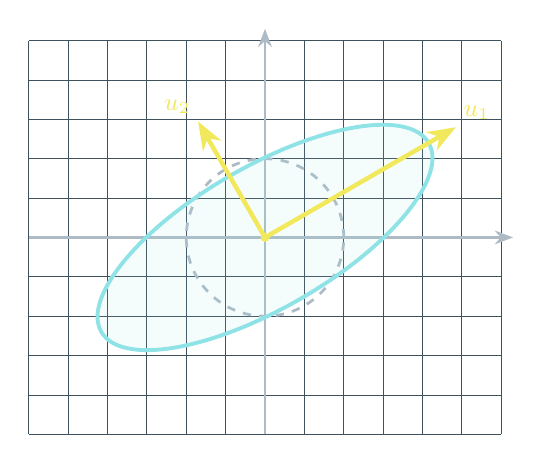
\begin{tikzpicture}[>=Stealth, font=\small]
  % 网格压在底层，颜色与背景接近，不抢图形
  \draw[step=0.5, gridc, line width=0.3pt] (-3,-2.5) grid (3,2.5);

  % 坐标轴
  \draw[axisc, line width=0.8pt, ->] (-3,0) -- (3.15,0);
  \draw[axisc, line width=0.8pt, ->] (0,-2.5) -- (0,2.65);

  % 原像：单位圆
  \draw[axisc, line width=1pt, dashed] (0,0) circle (1);

  % 像：长轴沿 30 度的椭圆
  \begin{scope}[rotate=30]
    \draw[ellipsec, line width=1.4pt, fill=ellipsec, fill opacity=0.10]
      (0,0) ellipse (2.4 and 0.9);
  \end{scope}

  % 两条正交主方向，与椭圆的长短轴严格重合
  \draw[accentc, line width=1.6pt, ->] (0,0) -- (30:2.8)
    node[above right, inner sep=2pt] {$u_1$};
  \draw[accentc, line width=1.6pt, ->] (0,0) -- (120:1.7)
    node[above left, inner sep=2pt] {$u_2$};

  \fill[accentc] (0,0) circle (1.6pt);
\end{tikzpicture}
\end{document}
